% Generated from the public primitive catalog. Original Atlas drawing; Apache-2.0.
% Target: ml-dsa; view: overview
\documentclass[border=9pt]{standalone}
% Original Atlas figure theme. Apache-2.0; see the repository LICENSE.
\usepackage[T1]{fontenc}
\usepackage{lmodern}
\usepackage{amsmath,amssymb}
\usepackage{tikz}
\usetikzlibrary{arrows.meta,positioning,calc,fit,backgrounds,decorations.pathreplacing,matrix}
\definecolor{atlasInk}{HTML}{172235}
\definecolor{atlasTeal}{HTML}{0D7B7D}
\definecolor{atlasMuted}{HTML}{637278}
\definecolor{atlasFill}{HTML}{EAF4F2}
\definecolor{atlasLine}{HTML}{B6C8C7}
\tikzset{
  every picture/.style={line width=.65pt,draw=atlasInk,>=Latex},
  every node/.style={text=atlasInk,font=\sffamily\small},
  box/.style={draw,rounded corners=1.5pt,minimum height=.9cm,minimum width=1.6cm,align=center,inner sep=6pt,fill=white},
  accent/.style={box,draw=atlasTeal,fill=atlasFill},
  wire/.style={->,line width=.7pt},
  keywire/.style={wire,draw=atlasTeal,dashed},
  xor/.style={draw,circle,fill=white,inner sep=0pt,minimum size=.38cm},
  add/.style={draw,rectangle,fill=white,inner sep=0pt,minimum size=.38cm},
  note/.style={font=\sffamily\scriptsize,text=atlasMuted,align=center},
  phase/.style={font=\sffamily\small\bfseries,text=atlasTeal},
  group/.style={draw=atlasLine,dashed,rounded corners=2pt,inner sep=8pt}
}
\newcommand{\rotl}{\mathbin{\lll}}
\newcommand{\rotr}{\mathbin{\ggg}}
\newcommand{\kx}{\operatorname{Keccak}\!\text{-}\!f[1600]}

\newcommand{\AtlasModulusBits}{b}
\newcommand{\AtlasFieldBits}{b}
\newcommand{\AtlasHash}{\textsf{H}}
\newcommand{\AtlasCurve}{\textsf{curve}}
\newcommand{\AtlasDhGroup}{\textsf{X25519 / X448}}
\newcommand{\AtlasDhPublicA}{\operatorname{XDH}(a,u_0)}
\newcommand{\AtlasDhPublicB}{\operatorname{XDH}(b,u_0)}
\newcommand{\AtlasDhSharedA}{\operatorname{XDH}(a,B)}
\newcommand{\AtlasDhSharedB}{\operatorname{XDH}(b,A)}
\newcommand{\AtlasSaltBytes}{s}
\newcommand{\AtlasSharedBits}{klen}
\newcommand{\AtlasPublicKeyBytes}{|pk|}
\newcommand{\AtlasSecretKeyBytes}{|sk|}
\newcommand{\AtlasCiphertextBytes}{|c|}
\newcommand{\AtlasSignatureBytes}{|\sigma|}
\newcommand{\AtlasModuleRank}{k}
\newcommand{\AtlasMatrixRows}{k}
\newcommand{\AtlasMatrixColumns}{\ell}
\newcommand{\AtlasHypertreeHeight}{h}
\newcommand{\AtlasHypertreeLayers}{d}
\newcommand{\AtlasForsHeight}{a}
\newcommand{\AtlasForsTrees}{k}
\newcommand{\AtlasHashBytes}{n}
\newcommand{\AtlasHashFamily}{\textsf{SHA2 / SHAKE}}
\begin{document}
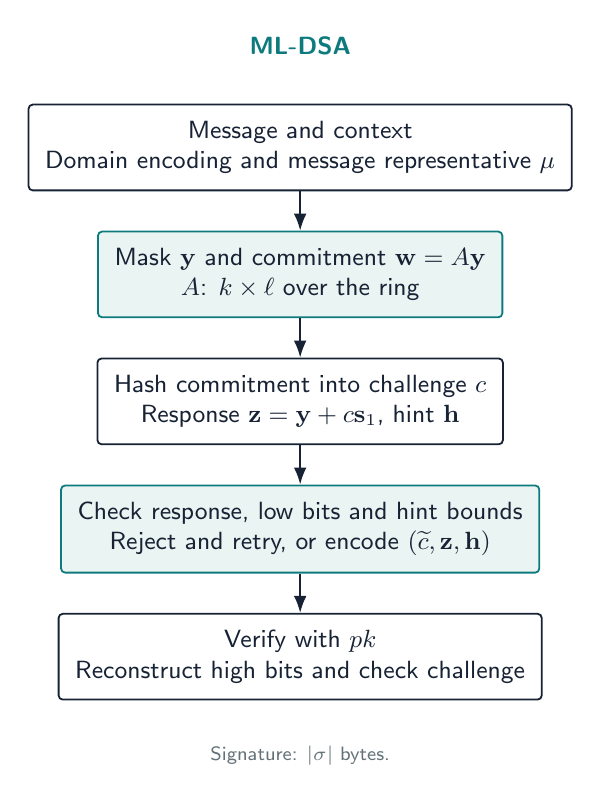
\begin{tikzpicture}[node distance=.5cm]
  \node[phase] (title) {ML-DSA};
  \node[box,below=of title] (input) {Message and context\\Domain encoding and message representative $\mu$};
  \node[accent,below=of input] (commit) {Mask $\mathbf y$ and commitment $\mathbf w=A\mathbf y$\\$A$: $\AtlasMatrixRows\times\AtlasMatrixColumns$ over the ring};
  \node[box,below=of commit] (response) {Hash commitment into challenge $c$\\Response $\mathbf z=\mathbf y+c\mathbf s_1$, hint $\mathbf h$};
  \node[accent,below=of response] (checks) {Check response, low bits and hint bounds\\Reject and retry, or encode $(\widetilde c,\mathbf z,\mathbf h)$};
  \node[box,below=of checks] (verify) {Verify with $pk$\\Reconstruct high bits and check challenge};
  \draw[wire] (input) -- (commit); \draw[wire] (commit) -- (response); \draw[wire] (response) -- (checks); \draw[wire] (checks) -- (verify);
  \node[note,below=.45cm of verify] {Signature: $\AtlasSignatureBytes$ bytes.};
\end{tikzpicture}

\end{document}
